\documentclass[envcountsect,runningheads]{llncs}

%%%%%%%%%%%%%%%%%%%%%%%%%%%%%%%%
% ENLARGED STYLE FOR SUBMISSION
%%%%%%%%%%%%%%%%%%%%%%%%%%%%%%%%
%\setlength{\textwidth}{15cm}
%\setlength{\textheight}{21cm}
%\addtolength{\oddsidemargin}{-1.25cm}
%\setlength{\evensidemargin}{\oddsidemargin}
%%%%%%%%%%%%%%%%%%%%%%%%%%%%%%%%

\usepackage[all]{xy}\CompileMatrices
\usepackage[english]{babel}
\usepackage[mathcal]{euscript}
\usepackage{latexsym}
\usepackage{amssymb}
\usepackage{pslatex}
\usepackage{alltt}

\usepackage{float}
%\usepackage{natbib}
\usepackage{url}
\usepackage{subfigure}
\usepackage{stmaryrd}
\usepackage{graphicx}
\graphicspath{ {images/} }

%new
\newcommand{\red}{\rightarrow}
\newcommand{\rred}{\Rightarrow}
\newcommand{\jeq}{\; \mathop{\triangleright} \;}
\def \mathrule #1#2#3{\begin{array}{l}%
    {\mbox{\scriptsize ({\sc #1})} }%
    \\ \irule{#2}{#3}%
\end{array}}
\newcommand{\irule}[2]{\frac{\textstyle\rule[-1.3ex]{0cm}{3ex}#1}%
{\textstyle\rule[-.5ex]{0cm}{3ex}#2}}
\newcommand{\pntrans}{[\rangle}
\newcommand{\arule}[3]{\frac{\textstyle\rule[-.8ex]{0cm}{3ex}#1}%
{\textstyle\rule[.2ex]{0cm}{3ex}#2}{\mbox{\scriptsize {\sc #3}}}}



% concurrency relation
\newcommand{\co}[1]{\mathbf{co}(#1)}
%symbol for depth function
\newcommand{\depth}{\ensuremath{\mathit{depth}}}
%symbol for natural numbers
\newcommand{\nat}{\ensuremath{\mathbb{N}}}
% category of persistent graph grammars
\newcommand{\pGG}{\ensuremath{\mathbf{PGG}}}
% category of persistent occurrence graph grammars
\newcommand{\poGG}{\ensuremath{\mathbf{POGG}}}
% category of prime event structures
\newcommand{\pes}{\mathbf{PES}}


%
% macros from Paolo Baldan's files
%
\newcommand{\elem}[1]{\ensuremath{\mathit{Elem}(#1)}}
% partial maps
\newcommand{\pto}{\rightarrowtail}
% domain of a partial map
\newcommand{\dom}[1]{\ensuremath{\mathit{dom}(#1)}}
% category of graphs with partial morphisms
\newcommand{\PGraph}{\ensuremath{\mathbf{PGraph}}}
% category of graphs with total morphisms
\newcommand{\Graph}{\ensuremath{\mathbf{Graph}}}
% typed graphs: underlying graph
\newcommand{\tgr}[1]{\ensuremath{|{#1}|}}
% typed graphs: underlying morphism
\newcommand{\tmap}[1]{\ensuremath{\tau_{{#1}}}}
% category of T-typed graphs with partial morphisms
\newcommand{\PTyped}[1]{\ensuremath{{#1}\mbox{-}\mathbf{PGraph}}}
% category of T-typed graphs with total morphisms
\newcommand{\Typed}[1]{\ensuremath{{#1}\mbox{-}\mathbf{Graph}}}
% unfolding functor for SPO grammars
\newcommand{\Unfs}{\ensuremath{\mathcal{U}_s}}
% functor from AES to O-GG
\newcommand{\Ngg}{\ensuremath{{\mathcal{N}}_s}}
% symbol for semi-abstract span
\newcommand{\spar}{\ensuremath{\leftrightarrow}}
% empty production
\newcommand{\emptyprod}{\ensuremath{\emptyset}}
% xypic label
\newcommand{\lb}[3]{\save []+<#2, #3>*\txt{\ensuremath{#1}}
  \restore}
% preconditions
\newcommand{\pre}[1]{\mbox{${^\bullet}\!{#1}$}}
% postconditions
\newcommand{\post}[1]{\mbox{${{#1} {^\bullet}}$}}
% contexts
\newcommand{\cont}[1]{\ensuremath{\underline{#1}}}
% strong causes
\newcommand{\cause}[1]{\ensuremath{\lfloor {#1} \rfloor }}
% weak dependency relation
\newcommand{\wc}{\ensuremath{\nearrow}}

% domain of a partial map
\newcommand{\pmapincluded}{\subseteq}

%
% FIGURE SEPARATOR
%
%\newcommand{\topfigrule}{\vskip3pt\noindent\rule{\textwidth}{1pt}\vskip-15pt}

%
% MACRO FOR COMMENTS
%
%\newcommand{\nota}[1]{\noindent \fbox{ \parbox{\textwidth}{#1} }  }
\newcommand{\nota}[1]{}

%
% ABBREVIATIONS AND SYMBOLS
%
\newcommand{\eg}{e.g.}
\newcommand{\ie}{i.e.}
\newcommand{\wrt}{w.r.t.}




%
% JOIN PROCESSES
%
\newcommand{\tuple}[1]{\vec{#1}}
\newcommand{\zero} {0}
\newcommand{\mess}[2] { #1 \langle #2 \rangle}
\newcommand{\defproc}[2]{\textrm{\bf def } #1 \textrm{ \bf in } #2}
\newcommand{\basdef}[2]{ #1\triangleright  #2}
\newcommand{\mergingdef}[2]{ #1 \blacktriangleright #2}
\newcommand{\begintrans}[3]{ #1\triangleright  [#2:#3]}
\newcommand{\trans}[2]{[#1:#2]}
\newcommand{\abort}{\mathit{abort}}
\newcommand{\bigpar}{|\!|}

\newcommand{\membrane}[1]{\{\![ #1 ]\!\}}

\newcommand{\denote}[1]{\llbracket #1\rrbracket}

\newcommand{\outp}[2]{\overline{#1}\langle #2 \rangle}
\newcommand{\inp}[2]{#1(#2)}


%Macros Hernan
\newcommand{\join}{\textsf {Join}}
\newcommand{\fn}{\mathit{fn}}
\newcommand{\dn}{\mathit{dn}}
\newcommand{\rn}{\mathit{rn}}
\newcommand{\subst}[2]{\{^{#1}/_{#2}\}}
\newcommand{\airlock}[2]{\triangleright}
\newcommand{\frozen}[1]{\llcorner #1 \lrcorner}
\newcommand{\reduce}{\rightarrow}
\newtheorem{notation}{Notation}



\title{A network computational model's for Software Defined Networking}
\author{Andr\'es Laurito}

\institute{
Departamento de Computac\'on - FCEN -UBA\\
 \email{andy.laurito@gmail.com} }

\titlerunning{A network computational model's for Software Defined Networking}

\authorrunning{A. Laurito}


\bibliographystyle{plain}

%%%%%%%%%%%%%%%%%%%%%%%%%%%%%%%%%%%%%%%%%%%%%%%%%%%%%%%%%%%%%%%%%
% DOCUMENT
%%%%%%%%%%%%%%%%%%%%%%%%%%%%%%%%%%%%%%%%%%%%%%%%%%%%%%%%%%%%%%%%%

\begin{document}

\maketitle

\begin{abstract}
 In this paper we define a computational model for netowrk's programming languages 
 In this paper we define a computational model for netowrk's programming languages 
 that use Software Defined Network (SDN) paradigm. For this purpose, 
 that use Software Defined Network (SDN) paradigm. For this purpose, 
 network's will be model as graphs, and a graph grammar semantic will be defined. 
 network's will be model as graphs, and a graph grammar semantic will be defined. 
 Production's in the grammar will model actions that can take place in the network, and programs 
 Production's in the grammar will model actions that can take place in the network, and programs 
 will be just a sequence of instruction's modifying a starting graph. \\
 will be just a sequence of instruction's modifying a starting graph. \\
 After graph grammar's definition, we will extend this grammar to a type graph grammar, and we 
 After graph grammar's definition, we will extend this grammar to a type graph grammar, and we 
 will explain how this new grammar can be applied to create a type programming language 
 will explain how this new grammar can be applied to create a type programming language 
 for networks. Finally we will show how this computational model is well defined, by using it to 
 for networks. Finally we will show how this computational model is well defined, by using it to 
 create a compiler for a new network progamming language recently emerged called Nemo.
 \end{abstract}

\section{Introduction}
Nowadays networks have became a crucial resource of any software application. 
Technologies for improving code crafting are emerging constantly. By contrast, network's have 
several issues to be solved. Some of this issues may be tagged as 
\begin{itemize}
  \item \textbf{Debugging problem's:} It is rather difficult to debug problems in network's using
  most known tools such as ping, traceroute, netstat, between others.
  \item \textbf{Changeability problem's:} changing traffic rule's, or 
security rule's in network may impliy modifying hundred, or even thousands code line's 
distributed in several devices around the network.
\item \textbf{Deployment problem's:} most changes are made mannually in several devices, 
making human mistakes easier.
\end{itemize}
Is it possible to do better ?, Can software be of help in this task?, Is it possible to know 
when network change's will break something before applying them?. \\
We believe that all this question's have possitive answers, and the best way of 
solving this problem nowadays is using network's programming languages which are 
build over the Software Defined Networking (SDN) paradigm.\\
Multiple SDN's programming languages have emerged over the past year's (some examples 
of these are Pyretic, Frenetic, Nemo, etc.), having each of them different approaches to solve 
some of the problems described before. Some of the principal lack's of the network 
programming languages discipline nowadays are formal grammar definitions, verification, 
validation, testing, software metrics and quality assurance, betwen multiple others. \\
Missing this properties makes harder to build some tools for network programming languages,
such as compiler's, debugger's, coding enviorment's, etc. This limitation's 
makes the network operator's job difficult, even when using some of this 
programming languages.\\
The main contribution of this paper is presenting, as far as the authors know, 
the first network computational model based on the definition of a graph 
grammar. In section 2 we will define the problem to be solved with several 
examples and assumptions. In section 3 we will define the graph grammar, and we 
will extend this grammar to a type graph grammar in section 4. In section 5 we 
will use this grammar to show how we can solve the problems specified in section 
2, and in section 6 we will check how the grammar can be used for building a 
simple compiler for the Nemo programming language. Finally, in section 7 we will 
give our conclusion and in section 8 we will introduce further work to be done.

\section{Definning the problem}
Let us remember that a program may be defined as a sequence of instruction's that executed 
perform a task in a computer or multiple computer's. Every program can be model as a Turing's 
machine or a finite lambda calculus computation, and despite of the model chosen, the 
operations are performed over a structure (usually this structure is a memory). In consequence,
every network program is model as a finite sequence of operations over a structure.\\
Our first proposal is to define this structure as an oriented graph, since network's 
can be easily mapped to graphs, and also is perfect reasonably to think 
program's operation as graph's rewriting. After this reasoning, the second propose is to define
a graph grammar in order to model all the network program's that may be written in any netowrk
programming language. \\
In order to define the grammar production's, we will narrow to model 
programs that solve the following problems in networks where each device support's SDN:\\
\\
\textbf{\underline{\textit{First Problem:}}} \\
Suppose that we have the following network:\\
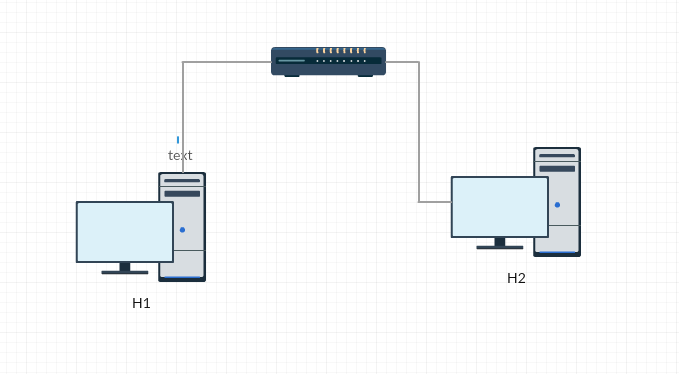
\includegraphics[width=\textwidth, height=8cm]{first_example.png}\\  
where H1 want's to establish an ssh 
connection with H2, and let's assume that there are not forwarding rules in 
order to establish such connection's, and also H2 has not an ssh server client to 
fullfilled this connection. \\
\\
\textbf{\underline{\textit{Second Problem:}}} \\
Suppose that we have the following network:\\
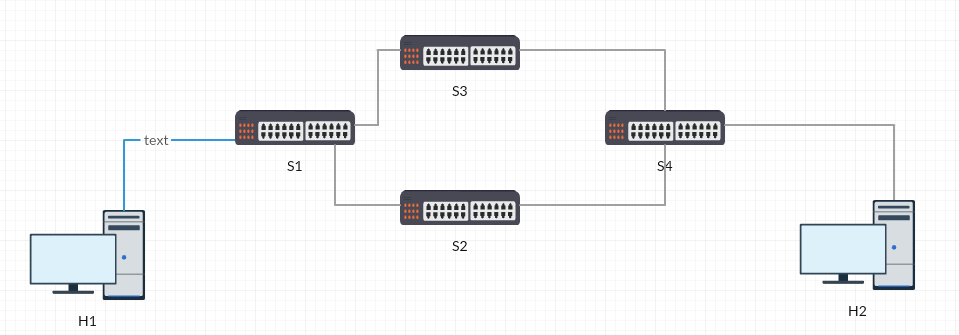
\includegraphics[width=\textwidth, height=8cm]{second_example.png}\\
where H1 wants to establish a ssh connection with H2, using S1->S2->S4 path, and 
let's assume that there are not forwarding rules from S2 to S4. 
\\

Defining a graph grammar allows us to check easily some of the problems described 
before, particularly static properties, such as examples 1 and 2 (as we will shall see in following
sections). However, dynamic properties (such as applying some load balancing policy when a 
queue start's to drop more than 50\% of packets) are not easily checked by grammar 
production's. Some problems required to execute our program in a traffic network, 
however our approach is identifying problems in program's before they actually 
happen in the real network. In order to identify this class of problems, we 
propose an execution of some of the grammar production's in a simulator which 
will be inserted inside the language compiler. The program will then be executed 
in several simulation's, in order to check if the production applied to the actual graph is 
possible. For doing this, we will mapped the dynamic grammar production's to 
devs (a formal language specification for defining simulator's), and we will run a simulation 
using this formal specification.\\
Having defined the problem that we will be solving, let's define the primitive 
operations that we will used in our computational model.

\section{Graph grammar production's}

We start by defining the most basic grammar production's. These 
productions are the one's that allows us to modify the network topoloy:


\begin{itemize}
  \item Creating a node
  \begin{figure}[H]
    \[
       \xymatrix@C=25pt@R=16pt
       {
         {}
         \POS[]-<4.5pc,0pc>\drop{NEW\_NODE:}
         \POS[]+<0pc,.5pc> *+=<3.8pc,3.8pc>[F-]{} & {\hookleftarrow} &
         {}
         \POS[]+<0pc,.5pc> *+=<3.8pc,3.8pc>[F-]{} & {\hookrightarrow} &
         {\bullet} \ar@(ul,ur)^{idle}
         \POS[]+<0pc,.5pc> *+=<3.8pc,3.8pc>[F-]{1} &
       }
    \]
    \caption{Creating a node}
    \protect\label{fig:nodecreation}
  \end{figure}
  This production creates a new logical node (this means that 
  the node could be either physic (which mean's it's a physical host with an 
  assocciated address) or logic (this mean's a group of physical nodes, meanning
  that the address could be a CIDR). \\
  It is important to remark that the created node is in an idle state, meaning 
  that is not interacting with any other node in the network. \\ 

  \item Deleting a node
  \begin{figure}[H]
    \[
       \xymatrix@C=35pt@R=16pt
       {
         {}\POS[]-<0pc,0pc>\drop{REMOVE\_NODE:}
         \\
         \\
         O \ar@(ul,ur)^{service} \POS[]-<1pc,.5pc>\drop{transmitter}&
         {\bullet} \ar@(ul,ur)^{idle} \ar@{.>}^{behaves}[l] \ar@{.>}^{behaves}[dl]
         \ar@{.>}^{source}[r] \ar@{.>}^{source}[dr] 
         \POS[]-<0pc,.5pc>\drop{1} &
         O \POS[]-<0pc,.5pc>\drop{link}
         \POS[]+<-5pc,-1pc> *+=<12pc,7pc>[F-]{} & {\hookleftarrow} &
         {}
         \POS[]+<0pc,.5pc> *+=<3.8pc,3.8pc>[F-]{} & {\hookrightarrow} &
         {}
         \POS[]+<0pc,.5pc> *+=<3.8pc,3.8pc>[F-]{} &
         \\
         O \ar@(r,d)^{service} \POS[]-<1pc,.5pc>\drop{receiver} & &
         O \POS[]-<0pc,.5pc>\drop{link}
       }
    \]
    \caption{Deleting a node}
    \protect\label{fig:nodedeletion}
  \end{figure}
  This is the production that will allow us to delete node's from our network. \\ 
  In order to apply this condition, we must satisfied that this node is neither 
  linked against a link, nor linked against a service.\\
  QUESTION: IS THE NEGATIVE CONDITION SAYING THAT ALL OF THIS PROPERTIES 
  MUST BE PRESENT TO NOT FULLFILLED THIS RULE?, OR IM SAYING THAT IF ONE OF
  THEM IS PRESENT, THEN IT FAILS (this is what I want).\\
   
  \item Node properties creation
  \begin{figure}[H]
    \[
       \xymatrix@C=25pt@R=16pt
       {
         {}\POS[]-<0pc,0pc>\drop{NODE\_PROPERTY\_CREATION:}
         \\
         \\
         O \ar@(ul,ur)^{property} \POS[]-<0pc,.5pc>\drop{prop} &
         {\bullet}_{1} \ar@(ul,ur)^{idle} \ar@{.>}^{has}[l]
         \POS[]+<-2pc,.5pc> *+=<6pc,3.8pc>[F-]{} & {\hookleftarrow} &
         {\bullet} \ar@(ul,ur)^{idle}
         \POS[]+<0pc,.5pc> *+=<3.8pc,3.8pc>[F-]{1} & {\hookrightarrow} &
         {\bullet}_{1} \ar@(ul,ur)^{idle} \ar@{->}^{has}[r]
         \POS[]+<1.5pc,.5pc> *+=<6pc,3.8pc>[F-]{} &
         {\bullet} \ar@(ul,ur)^{property} \POS[]-<0pc,.5pc>\drop{prop}
       }
    \]
    \caption{Node properties creation}
    \protect\label{fig:nodecreation}
  \end{figure}
  This production allows us to create a node's property. The only condition to 
  be satisfied to apply this production, is that the property to be created can't be an already
  defined property for node 1.
  
  \item Node properties deletion
  \begin{figure}[H]
    \[
       \xymatrix@C=25pt@R=16pt
       {
         {}\POS[]-<0pc,0pc>\drop{NODE\_PROPERTY\_DELETION:}
         \\
         \\
         {\bullet} \ar@(ul,ur)^{property} \POS[]-<0pc,.5pc>\drop{prop} &
         {\bullet}_{1} \ar@(ul,ur)^{idle} \ar@{->}^{has}[l]
         \POS[]+<-2pc,.5pc> *+=<6pc,3.8pc>[F-]{} & {\hookleftarrow} &
         {\bullet} \ar@(ul,ur)^{idle}
         \POS[]+<0pc,.5pc> *+=<3.8pc,3.8pc>[F-]{1} & {\hookrightarrow} &
         {\bullet}_{1} \ar@(ul,ur)^{idle}
         \POS[]+<0pc,.5pc> *+=<3.8pc,3.8pc>[F-]{}
       }
    \]
    \caption{Node properties deletion}
    \protect\label{fig:nodedeletion}
  \end{figure}
  This production allows us to remove a node's property. At first, I see no need 
  to impose some restriction to applied this rule.\\
  
  \item Service Creation
  \begin{figure}[H]
    \[
       \xymatrix@C=35pt@R=16pt
       {
        {}
         \POS[]-<5pc,0pc>\drop{NEW\_SERVICE:}
         \POS[]+<0pc,.5pc> *+=<3.8pc,3.8pc>[F-]{} & {\hookleftarrow} &
         {}
         \POS[]+<0pc,.5pc> *+=<3.8pc,3.8pc>[F-]{} & {\hookrightarrow} &
         {\bullet} \ar@(ul,ur)^{service} \ar@{->}^{dual}[r] \POS[]-<-0.5pc,.5pc> \drop{transmitter} 
         &
         {\bullet} \ar@(ul,ur)^{service} \POS[]-<-0.5pc,.5pc> \drop{receiver}
         \POS[]+<-2pc,.5pc> *+=<7.5pc,3.8pc>[F-]{} &
      }
    \]
    \caption{Service Creation}
    \protect\label{fig:servicecreation}
  \end{figure}
  In this production we define a new service. A service is either some property 
  implemented in nodes, or implemented in another node, wich will be used for generating 
  flows,this means that, when a flow is created, this flow will be of type service. The fact that the
  main idea is to send and receive information, is represented as dual nodes representing a 
  transmitter and a reicever in the graph.\\
  
  \item Service Deletion
  \begin{figure}[H]
    \[
       \xymatrix@C=35pt@R=16pt
       {
        {} \POS[]-<0pc,0pc>\drop{REMOVE\_SERVICE:}
         \\
         \\
         {\bullet} \ar@(ul,ur)^{service} \ar@{->}^{dual}[r]
         \POS[]-<-0.5pc,.5pc> \drop{transmitter} 
         &
         {\bullet} \ar@(ul,ur)^{service} \POS[]-<-0.5pc,.5pc> \drop{receiver}
         & {\hookleftarrow} &
         {}
         \POS[]+<0pc,.5pc> *+=<3.8pc,3.8pc>[F-]{} & {\hookrightarrow} &
         {}
         \POS[]+<0pc,.5pc> *+=<3.8pc,3.8pc>[F-]{}
         \\
         {\bullet} \ar@(r,d)^{idle} \ar@{.>}^{behaves}[u] \POS[]-<-0.5pc,.5pc> \drop{1} &
         {\bullet} \ar@(r,d)^{idle} \ar@{.>}^{behaves}[u] \POS[]-<-0.5pc,.5pc> \drop{2}
         \POS[]+<-2pc,1pc> *+=<8pc,7pc>[F-]{}
      }
    \]
    \caption{Service Creation}
    \protect\label{fig:servicecreation}
  \end{figure}
  In this production we remove a service, whenever the service is not attached by a node.\\
  
  \item Node behaves as some endpiont of communication
  \begin{figure}[H]
    \[
       \xymatrix@C=35pt@R=35pt
       {
         {}\POS[]-<1pc,0pc>\drop{NODE\_IMPLEMENTS\_ROLE:}
         \\
         {\bullet}_{1} \ar@(ul,ur)^{idle} &
         {\bullet} \ar@(ul,ur)^{service} \ar@{->}^{dual}[d] \POS[]-<-0.5pc,.5pc> \drop{transmitter}
         & {\hookleftarrow} &
         {\bullet}_{1} \ar@(ul,ur)^{idle} &
         {\bullet} \ar@(ul,ur)^{service} \ar@{->}^{dual}[d] \POS[]-<-0.5pc,.5pc> \drop{transmitter}
         & {\hookrightarrow} &
         {\bullet}_{1} \ar@(ul,ur)^{idle}\ar@{->}^{behaves}[r]
         &
         {\bullet} \ar@(ul,ur)^{service} \ar@{->}^{dual}[d] \POS[]-<-0.5pc,.5pc> \drop{transmitter}
         \\
         & {\bullet} \ar@(r,d)^{service} \POS[]-<1.5pc,0pc> \drop{receiver}
         \POS[]+<-1pc,2pc> *+=<7.5pc,9pc>[F-]{} & & &
         {\bullet} \ar@(r,d)^{service} \POS[]-<1.5pc,0pc> \drop{receiver}
         \POS[]+<-1pc,2pc> *+=<7.5pc,9pc>[F-]{} & & &
         {\bullet} \ar@(r,d)^{service} \POS[]-<1.5pc,0pc> \drop{receiver}
         \POS[]+<-1pc,2pc> *+=<7.5pc,9pc>[F-]{}
       }
    \]
    \caption{Node implements role}
    \protect\label{fig:attachmentnodetoservice}
  \end{figure}
  This production is used to make node's to behave as one of the endpoints in 
  the communication of services. One node could eventually behave as either 
  endpoints (an example of this situation could be a http connection, where the node is 
  both client and server).\\

 \item Node stops behaving as some endpiont in the communication
  \begin{figure}[H]
    \[
       \xymatrix@C=35pt@R=35pt
       {
         {}\POS[]-<1pc,0pc>\drop{NODE\_STOPS\_IMPLEMENTING\_ROLE:}
         \\
         {\bullet}_{1} \ar@(ul,ur)^{idle} \ar@{->}^{behaves}[r] &
         {\bullet} \ar@(ul,ur)^{service} \ar@{->}^{dual}[d] \POS[]-<-0.5pc,.5pc> \drop{transmitter}
         & {\hookleftarrow} &
         {\bullet} \ar@(ul,ur)^{service} \ar@{->}^{dual}[d]  \POS[]-<-0.5pc,.5pc> \drop{transmitter}
         & {\hookrightarrow} &
         {\bullet} \ar@(ul,ur)^{service} \ar@{->}^{dual}[d] \POS[]-<-0.5pc,.5pc> \drop{transmitter}
         \\
         & {\bullet} \ar@(r,d)^{service} \POS[]-<1.5pc,0pc> \drop{receiver}
         \POS[]+<-1pc,2pc> *+=<7.5pc,9pc>[F-]{} & 
         & {\bullet} \ar@(r,d)^{service} \POS[]-<1.5pc,0pc> \drop{receiver}
         \POS[]+<0pc,2pc> *+=<6pc,9pc>[F-]{} &
         & {\bullet} \ar@(r,d)^{service} \POS[]-<1.5pc,0pc> \drop{receiver}
         \POS[]+<0pc,2pc> *+=<6pc,9pc>[F-]{}
       }
    \]
    \caption{Node stops implementing role}
    \protect\label{fig:deattachmentnodetoservice}
  \end{figure}
  This production is used to make a node stop behaving as one of the communication's 
  endpoint.\\
  I THINK THIS SHOULD BE THE STANDARD TO USE FOR EVERY PRODUCTION THAT DELETES
  PROPERTIES OR NODES FROM GRAPH (REMEMBER THAT SERVICES, NODES CAN STOP 
  WORKING WHILE THE NETWORK IS RUNNING).\\
   
  \item Link creation
  \begin{figure}[H]
    \[
       \xymatrix@C=25pt@R=16pt
       {
        {\bullet}_{1}\ar@(ul,ur)^{idle} \ar@{.>}^{source}[d]
        \POS[]-<3.8pc,0pc>\drop{NEW\_LINK:} &
         {\bullet}_{2}\ar@(ul,ur)^{idle}\ar@{.>}^{target}[dl]
         & {\hookleftarrow} &
         {\bullet}_{1}\ar@(ul,ur)^{idle} &
         {\bullet}_{2}\ar@(ul,ur)^{idle}
         \POS[]+<-2pc,-.5pc>*+=<7pc,8pc>[F-]{} & {\hookrightarrow} &
         {\bullet}_{1}\ar@(ul,ur)^{idle} \ar@{->}^{source}[d] &
         {\bullet}_{2} \ar@(ul,ur)^{idle}\ar@{->}^{target}[dl]
         \\
         O \POS[]-<.8pc,0pc> \drop{link}
         \POS[]+<2pc,2pc>*+=<7pc,8pc>[F-]{} & & & & & &
         {\bullet}_{link} 
         \POS[]+<2pc,2pc>*+=<7pc,8pc>[F-]{} 
       }
    \]
    \caption{Link creation}
    \protect\label{fig:linkcreation}
  \end{figure}
  Here we define a new link between nodes 1 and 2. The only condition to apply 
  this production is that both nodes must be in an idle state and neither of them should have an 
  existing link between them. This restriction is denoted by the dot lined in L, 
  wich represents the negative condition.\\
  Note: Being in an idle state does not mean that they are doing nothing!. An 
  idle state behaves likes a wildcard, meaning that from this state, multiply actions 
  can be applied to the node.\\
  
  \item Link deletion
  \begin{figure}[H]
    \[
       \xymatrix@C=25pt@R=16pt
       {
        {\bullet}_{1}\ar@(ul,ur)^{idle} \ar@{->}^{source}[d]
        \POS[]-<5pc,0pc>\drop{REMOVE\_LINK:} &
         {\bullet}_{2}\ar@(ul,ur)^{idle}\ar@{->}^{target}[dl]
         & {\hookleftarrow} &
         {\bullet}_{1}\ar@(ul,ur)^{idle} &
         {\bullet}_{2}\ar@(ul,ur)^{idle}
         \POS[]+<-2pc,-.5pc>*+=<7pc,8pc>[F-]{} & {\hookrightarrow} &
         {\bullet}_{1}\ar@(ul,ur)^{idle} &
         {\bullet}_{2} \ar@(ul,ur)^{idle}
         \POS[]+<-2pc,-.5pc>*+=<7pc,8pc>[F-]{}
         \\
         {\bullet} \POS[]-<.8pc,0pc> \drop{link}
         \POS[]+<2pc,2pc>*+=<7pc,8pc>[F-]{} 
       }
    \]
    \caption{Link deletion}
    \protect\label{fig:linkdeletion}
  \end{figure}
  This is the production used to remove links from nodes. When we allow this production to be
  applied without contraints, we are trying to represent real states that could happen, since 
  links usually fail witout previous warning.\\
  
  \item Link's property creation
  \begin{figure}[H]
    \[
       \xymatrix@C=25pt@R=16pt
       {
         {}\POS[]+<0pc,2pc>\drop{NEW\_LINK\_PROPERTY:}
         \\
         {\bullet}\ar@(ul,ur)^{property} \POS[]-<0pc,.5pc>\drop{prop} & 
         {\bullet} \ar@{.>}^{has}[l] \POS[]-<0pc,.5pc>\drop{link}
         \POS[]+<-2pc,.5pc> *+=<6pc,3.8pc>[F-]{} 
         & {\hookleftarrow} &
         {\bullet}\POS[]-<0pc,.5pc>\drop{link}
         \POS[]+<0pc,.5pc> *+=<3.8pc,3.8pc>[F-]{} & {\hookrightarrow} &
         {\bullet}\ar@{->}^{has}[r]\POS[]-<0pc,.5pc>\drop{link}
         \POS[]+<2.5pc,.5pc> *+=<7.5pc,3.8pc>[F-]{} &
         {\bullet}\ar@(ul,ur)^{property}
         \POS[]+<0pc,.5pc>*+=<3pc,3pc>[]{}\POS[]-<0pc,.8pc>\drop{prop}
       }
    \]
    \caption{Link's property creation}
    \protect\label{fig:linkpropertycreation}
  \end{figure}
  As in the node's creation property, this production allows us to create a new 
  link's property. The condition to be satisfied to apply this production, is 
  that link cannot have defined the property to be created.
  This properties are going to be 
  perhaps physical properties in physical links (for example, we can define here bandwith, 
  average latency, perhpahs if it's either ethernet or wifi), and some other properties in logical 
  nodes.\\
  QUESTIONS:\\
  1) What properties could be assigned to a logical link? \\
  2) Can I always define properties in a node? (It really doesn't matter what is going on with 
  that link in the network?. Perphas it happens something similar as nodes, that we need some 
  'idle' state, for example, an empty state).\\
  
  \item Link's property deletion
  \begin{figure}[H]
    \[
       \xymatrix@C=25pt@R=16pt
       {
         {}\POS[]+<0pc,2pc>\drop{REMOVE\_LINK\_PROPERTY:}
         \\
         {\bullet}\ar@(ul,ur)^{property} \POS[]-<0pc,.5pc>\drop{prop} & 
         {\bullet} \ar@{->}^{has}[l] \POS[]-<0pc,.5pc>\drop{link}
         \POS[]+<-2pc,.5pc> *+=<6pc,3.8pc>[F-]{} 
         & {\hookleftarrow} &
         {\bullet}\POS[]-<0pc,.5pc>\drop{link}
         \POS[]+<0pc,.5pc> *+=<3.8pc,3.8pc>[F-]{} & {\hookrightarrow} &
         {\bullet}\POS[]-<0pc,.5pc>\drop{link}
         \POS[]+<0pc,.5pc> *+=<3.8pc,3.8pc>[F-]{} 
       }
    \]
    \caption{Link's property deletion}
    \protect\label{fig:linkpropertydeletion}
  \end{figure}
  This is the production that allows us to remove properties from a link.\\
  
  \end{itemize}
  
  So far we have defined productions that are intended to be use between the interactions 
  with the elements in the network. With the following productions, we will start using the productions
  listed before, in order to crate interaction between the elements in the network. \\
  
  \begin{itemize}
    \item Flow creation
  \begin{figure}[H]
    \[
       \xymatrix@C=25pt@R=35pt
       {
         {}\POS[]-<1pc,0pc>\drop{NEW\_FLOW:}
         \\
         {\bullet} \POS[]-<.5pc,.5pc> \drop{link} &
         {\bullet}_{1} \ar@(ul,ur)^{idle} \ar@{->}^{behaves}[r] \ar@{->}^{source}[l] &
         {\bullet} \ar@(ul,ur)^{service} \ar@{->}^{dual}[d] \POS[]-<-0.5pc,.5pc> \drop{transmitter}
         & {\hookleftarrow} &
         {\bullet} \POS[]-<.5pc,.5pc> \drop{link} &
         {\bullet}_{1} \ar@(ul,ur)^{idle} \ar@{->}^{behaves}[r] \ar@{->}^{source}[l] &
         {\bullet} \ar@(ul,ur)^{service} \ar@{->}^{dual}[d] \POS[]-<-0.5pc,.5pc> \drop{transmitter}
         & {\hookrightarrow} &
         {\bullet} \POS[]-<1pc,.5pc> \drop{link} &
         {\bullet}_{1} \ar@(ul,ur)^{idle}\ar@{->}^{behaves}[r] \ar@{->}^{source}[l]
         &
         {\bullet} \ar@(ul,ur)^{service} \ar@{->}^{dual}[d] \POS[]-<-0.5pc,.5pc> \drop{transmitter}
         \\
         &
         {\bullet}_{2} \ar@(ul,ur)^{idle}\ar@{->}^{behaves}[r] \ar@{->}^{target}[ul] & 
         {\bullet} \ar@(r,d)^{service} \POS[]-<-1.5pc,0pc> \drop{receiver}
         \POS[]+<-2.5pc,2pc> *+=<10pc,9pc>[F-]{} & & &
         {\bullet}_{2} \ar@(ul,ur)^{idle}\ar@{->}^{behaves}[r] \ar@{->}^{target}[ul] & 
         {\bullet} \ar@(r,d)^{service} \POS[]-<-1.5pc,0pc> \drop{receiver}
         \POS[]+<-2.5pc,2pc> *+=<10pc,9pc>[F-]{} & &
         {\bullet} \ar@(r,d)^{running} \ar@{->}^{over}[u] \POS[]-<1pc,0pc> \drop{flow} &
         {\bullet}_{2} \ar@(ul,ur)^{idle}\ar@{->}^{behaves}[r] \ar@{->}^{target}[ul] & 
         {\bullet} \ar@(r,d)^{service} \POS[]-<-1.5pc,0pc> \drop{receiver}
         \POS[]+<-3pc,2pc> *+=<11pc,9pc>[F-]{}
       }
    \]
    \caption{Flow creation}
    \protect\label{fig:flowcreation}
  \end{figure}
  In order to create a flow, I first need two things: 
  \begin{itemize}
    \item I need to have a link between the nodes
    \item One node has to behave as the transmitter, while the other one should 
    behave as the reicever.  
   \end{itemize}
  
  Lets go through these rules one more time. The first rule is just telling us that, in order to be 
  able to
  create a node, I need a connection between this node's (remember that this conection can be either
  logical or physical).\\
  The second rule is telling us that, in order to create a flow of type X (lets say for example, 
  that I want to create a ssh flow between this nodes), I need to guarantee that 
  both nodes implements the same service, and one transmits while the other 
  listens.\\
  Finally, it's important to notice that the new flow is created in a running state, 
  and is associated to the link with the link over, meaning that the flow is running over 
  this link. \\
  \\
  THINS THAT HAD TO BE THINK A BIT MORE: \\
  1) Some rules may not be valid in this context ... ¿How do I deny multiple ssh 
  conections betwen same nodes? (Also, this sounds to me like a type condition, since another
  services may allow this behaviour, for example sql.) \\
 
 \item Remove flow from link
  \begin{figure}[H]
    \[
       \xymatrix@C=35pt@R=35pt
       {
         {}\POS[]-<1pc,0pc>\drop{REMOVE\_FLOW\_FROM\_LINK:}
         \\
         {\bullet} \POS[]-<-0.5pc,.5pc> \drop{link}
         & {\hookleftarrow} &
         {\bullet} \POS[]-<-0.5pc,.5pc> \drop{link}
         & {\hookrightarrow} &
         {\bullet} \POS[]-<-0.5pc,.5pc> \drop{link}
         \\
         {\bullet} \ar@(r,d)^{running} \ar@{->}^{over}[u] \POS[]-<1.5pc,0pc> \drop{flow} 
         \POS[]+<0pc,2pc> *+=<5pc,9pc>[F-]{} & &
          {}
         \POS[]+<0pc,2pc> *+=<5pc,9pc>[F-]{} & &
         {}
         \POS[]+<0pc,2pc> *+=<5pc,9pc>[F-]{}
       }
    \]
    \caption{Remove flow from link}
    \protect\label{fig:removeflowfromlink}
  \end{figure}
  This production is used to remove flows from links. Notice that is not necessary to detach 
  nodes from services, since they can still create new flows from the services where they 
  are attached. This production could be used for example, when a flow ends.\\
 
  \item Flow's property creation
  \begin{figure}[H]
    \[
       \xymatrix@C=25pt@R=16pt
       {
         {}\POS[]-<0pc,0pc>\drop{FLOW\_PROPERTY\_CREATION:}
         \\
         \\
         O \ar@(ul,ur)^{property} \POS[]-<0pc,.5pc>\drop{prop} &
         {\bullet}_{flow} \ar@(ul,ur)^{running} \ar@{.>}^{has}[l]
         \POS[]+<-2pc,.5pc> *+=<6pc,3.8pc>[F-]{} & {\hookleftarrow} &
         {\bullet}_{flow} \ar@(ul,ur)^{running}
         \POS[]+<0pc,.5pc> *+=<3.8pc,3.8pc>[F-]{} & {\hookrightarrow} &
         {\bullet}_{flow} \ar@(ul,ur)^{running} \ar@{->}^{has}[r]
         \POS[]+<1.5pc,.5pc> *+=<6pc,3.8pc>[F-]{} &
         {\bullet} \ar@(ul,ur)^{property} \POS[]-<0pc,.5pc>\drop{prop}
       }
    \]
    \caption{Node properties creation}
    \protect\label{fig:nodecreation}
  \end{figure}
  As other productions already defined, this one allow's us to create a new 
  flow's property. The only condition to be satisfied, is that this new property 
  to be created is not already created in flow.
  
  QUESTIONS:\\
  1) Can this properties be the actions associated in the nemo language ? 
  Perphaps properties can be understood as premises that have to be guaranteed 
  while the flow exist. \\
  2) Some of this properties could be dynamic (this has sense, since flow is the representation 
  of dynamism in the network). \\

  \item Flow's property deletion
  \begin{figure}[H]
    \[
       \xymatrix@C=25pt@R=16pt
       {
         {}\POS[]-<0pc,0pc>\drop{REMOVE\_FLOW\_PROPERTY:}
         \\
         \\
         {\bullet} \ar@(ul,ur)^{property} \POS[]-<0pc,.5pc>\drop{prop} &
         {\bullet}_{flow} \ar@(ul,ur)^{running} \ar@{->}^{has}[l]
         \POS[]+<-2pc,.5pc> *+=<6pc,3.8pc>[F-]{} & {\hookleftarrow} &
         {\bullet}_{flow} \ar@(ul,ur)^{running}
         \POS[]+<0pc,.5pc> *+=<3.8pc,3.8pc>[F-]{} & {\hookrightarrow} &
         {\bullet}_{flow} \ar@(ul,ur)^{running}
         \POS[]+<0pc,.5pc> *+=<3.8pc,3.8pc>[F-]{} 
       }
    \]
    \caption{Flow properties deletion}
    \protect\label{fig:flowpropertydeletion}
  \end{figure}
  Finally, this productions allows us to remove properties from a flow.
   
\end{itemize} 

\section{Graph instantiation}

In this section we will focus in giving several examples of the usage of the 
grammar recently defined. The examples used in this section will be those defined in 
a previous document (REMEMBER TO REWRITE EXAMPLES HERE) \\ 
Lets first defined the first example, a network with two host and a router, 
which want to start a ssh connection. \\
There were two problems here:
\begin{itemize}
  \item Neither of the host had ssh active
  \item Neither of the host were connected to the router.
\end{itemize}

Let's model our network, and see how the grammar defined before help us to 
detect problems in what we are trying to do.\\
This would be the network represented in our model:
\begin{figure}[H]
    \[
       \xymatrix@C=25pt@R=30pt
       {
         {}\POS[]-<0pc,0pc>\drop{FIRST EXAMPLE}
         \\
         \\
         {\bullet}\ar@(ul,ur)^{idle} \POS[]-<-.5pc,.5pc> \drop{h1} &
         {\bullet}\ar@(ul,ur)^{idle} \POS[]-<-.5pc,.5pc> \drop{router} &
         {\bullet}\ar@(ul,ur)^{idle} \POS[]-<-.5pc,.5pc> \drop{h2}
      }
    \]
\end{figure}

Having model our network, what we can check is that NEW\_FLOW production can't be 
applied to my network (since there is no morphism between the left side of the production 
and this model). In this case, if I write a program for the situation described, 
we will have a compiler error, since there's going to be an instruction that 
cannot be done, and this is because the production associated with it cannot be 
executed.

\end{document}
